\documentclass[11pt]{article}
\usepackage{geometry}

\usepackage{amsmath}
\usepackage{amssymb}
\usepackage{enumerate}
\usepackage{epsfig}
\usepackage{graphicx}
\graphicspath{{./fig/}}
\usepackage{hyperref}
\usepackage{relsize}
\usepackage{url}

% For apa-style bibliography
\usepackage[nosectionbib]{apacite}
\bibliographystyle{apacite}

% For R code snippets
\usepackage{listings}

% Custom math shortcuts for expressions used many times throughout the paper
\newcommand{\Rsq}{$R^2\,$}
\newcommand{\boldrho}{\boldsymbol{\rho}}
\newcommand{\boldbeta}{\boldsymbol{\beta}}
\newcommand{\boldtheta}{\boldsymbol{\theta}}
\newcommand{\boldeps}{\boldsymbol{\epsilon}}
\newcommand{\hatbeta}{\widehat{\boldbeta}}
\newcommand{\hatalpha}{\widehat{\alpha}}
\newcommand{\sigmaEps}{\sigma_{\epsilon}}
\newcommand{\X}{\mathbf{X}}
\newcommand{\y}{\mathbf{y}}
\newcommand{\Q}{\mathbf{Q}}
\newcommand{\R}{\mathbf{R}}
\renewcommand{\u}{\mathbf{u}}
\newcommand{\locRsq}{\ell_{R^2}}
\newcommand{\halfK}{\frac{K}{2}}
\newcommand{\Betadist}[2]{\mathsf{Beta}\left(#1,#2\right)}
\newcommand{\Digamma}[1]{\psi\left(#1\right)}
\newcommand{\given}{\left.\right|}
\newcommand{\draw}{{(s)}}

%: Title, authors, date
\title{\bf Regularizing Bayesian linear models with an informative prior on \Rsq
    \vspace{.1in}}
\author{Ben Goodrich\footnote{Columbia University, New York.}
    \and Jonah Gabry$^\ast$
    \and Andrew Gelman$^\ast$
    \vspace{.1in}}
    \vspace{-.2in}}

%: Begin document
\begin{document}
\maketitle
\thispagestyle{empty}

\begin{abstract}
\noindent We derive an approach for expressing prior beliefs about the location
of the \Rsq, the familiar proportion of variance in the outcome variable that is
attributable to the predictors under a linear model. In particular, when there
are many predictors relative to the number of observations we would expect the
joint prior derived here to work better than placing independent, heavy-tailed
priors on the coefficients, which is  standard practice in applied Bayesian data
analysis but neither reflects the beliefs of the researcher nor conveys enough
information to stabilize all the computations.
\end{abstract}


\section{Introduction}

Fully making Bayesian estimation of linear models routine for applied
researchers requires prior distributions that work well for any data generated
according to the assumptions of the likelihood function. Most Bayesian
approaches require the researcher to specify a joint prior distribution for the
regression coefficients (and the intercept and error variance), but most applied
researchers have little inclination to specify all of these prior distributions
thoughtfully and take a shortcut by specifying a single prior distribution that
is taken to apply to all regression coefficients as if they were independent of
each other (and the intercept and error variance).

In this paper we derive and demonstrate an approach for directly expressing
prior beliefs about the location of the \Rsq, the familiar proportion of
variance in the outcome variable that is attributable to the predictors under a
linear model. Our work shares some common themes with other research. For
example, \citeA{guan-stephens} proposes a sparcity-inducing prior on the
coefficients of a linear model that has implications for the \Rsq. In
particular, their prior relaxes the assumption of prior independence between the
parameter representing the typical magnitude of the non-zero coefficients and
the parameter governing sparcity, which allows for the a priori expectation that
the proportion of variance explained does not necessarily increase markedly with
model complexity.

Our approach results in a regularizing prior on the coefficients but does not
induce sparcity in the sense of setting coefficients equal to exactly zero. The
degree of shrinkage depends on the number of estimated effects and, in
particular, on prior information provided by the researcher about \Rsq. Since
the \Rsq is a well-understood bounded scalar it is easy to specify prior
information about it and, for most applied problems, researchers will have
enough familiarity with their subject matter to have some a priori knowledge
about the extent to which their predictors will account for variation in the
outcome. In particular, when there are many predictors relative to the number of
observations we would expect the joint prior derived here to work better than
placing independent, heavy-tailed priors on the regression coefficients in the
linear model, which neither reflects the beliefs of the researcher nor conveys
enough information to stabilize all the computations.

The paper is organized as follows. We begin in Section~\ref{sec:likelihood} with
a brief review of the linear model with a QR decomposition applied to the design
matrix. Section~\ref{sec:priors} covers the specification of our proposed joint
prior distribution for the parameters in the QR-reparameterized model. In
Section~\ref{sec:posterior} we show how to recover the parameters of interest
from the posterior distribution of the primitive parameters of the
reparameterized model. Finally, in Section~\ref{sec:example} we demonstrate our
implementation of the proposed model in the {\tt rstanarm} R package and then
conclude with a brief discussion of possible extensions to the work presented
here.


\section{QR-reparameterized likelihood}
\label{sec:likelihood}

The likelihood contribution for one observation $y_i$ under a linear model
can be written as the conditional normal density
%
$$
f \left(y_i \given \mu_i, \sigmaEps \right) =
\mathsf{Normal}\left(y_i \given \mu_i, \sigmaEps \right) =
\frac{1}{\sigmaEps \sqrt{2 \pi}} \,
\exp{\left\{-\frac{1}{2} \left(\frac{y_i - \mu_i}{\sigmaEps}\right)^2\right\}},
$$
%
where $\mu_i = \alpha + \mathbf{x}_i^\top \boldbeta$ is a linear predictor and
$\sigmaEps$ is the standard deviation of the error in predicting the outcome.
For a sample of size $N$, the likelihood of the entire sample is the product of
the $N$ individual likelihood contributions, and it is well known that it is
maximized when the sum of squared residuals is minimized. This occurs when
%
\begin{align*}
\hatbeta &= \left(\X^\top \X \right)^{-1} \X^\top \y,\\
\hatalpha &= \overline{y} - \overline{\mathbf{x}}^\top \hatbeta,\\
\widehat{\sigma}_{\epsilon}^2 &=
  \frac{1}{N}
  \left(\y - \hatalpha - \X \hatbeta \right)^\top
  \left(\y - \hatalpha - \X \hatbeta \right),
\end{align*}
%
where $\overline{\mathbf{x}}$ is a vector of sample means for the
$K$ predictors, $\X$ is a $N \times K$ matrix of \emph{centered} predictors,
$\y$ is a $N$-vector of outcomes, and $\overline{y}$ is the sample mean of the
outcome.

Taking a QR decomposition of the centered design matrix, $\X = \Q\R$, where
$\Q^\top \Q = \mathbf{I}$ and $\R$ is upper triangular, we can write the maximum
likelihood estimate for the regression coefficients --- the least squares
solution --- as
%
$$\hatbeta = \left(\X^\top \X \right)^{-1} \X^\top \y = \R^{-1} \Q^\top \y.$$
%
It is helpful for intuition to notice that when substituting $\Q\R$ for $\X$
in the linear model we obtain another linear model
%
$$\y = \X\boldbeta + \boldeps \implies \y = \Q\boldtheta + \boldeps,$$
%
where the relationship between $\boldbeta$ and $\boldtheta$ is given by
%
$$\boldbeta = \R^{-1}\boldtheta.$$
%
That is, we have moved from a regression of $\y$ on $\X$ to a regression of
$\y$ on the orthogonal matrix $\Q$.

The QR decomposition is often used in this way for improved numerical stability
(as in the familiar {\tt lm} function in R), but, as we outline below, it is
also useful for thinking about priors in a Bayesian version of the linear model.


\section{Specification of the joint prior distribution}
\label{sec:priors}

The key innovation in this paper is the prior for the parameters in the
QR-reparameterized model. To understand this prior, we start with the equations
that characterize the maximum likelihood solutions \emph{before} observing the
data $\left(\y, \X\right)$.

Let $\boldtheta = \R\boldbeta = \Q^\top \y$ and $\Q_k$ denote the $k$th column
of $\Q$. We can write the $k$th element of the vector $\boldtheta$ as
$$\theta_k
  = {\rm Corr}(\y, \Q_k) \, \frac{{\rm sd}(\y)}{{\rm sd}(\Q_k)}
  = \rho_k \, \sigma_y \, \sqrt{N - 1},
$$
where $\rho_k$ is the correlation between $\Q_k$ and the outcome, $\sigma_y$ is
the marginal standard deviation of the outcome, and $1/\sqrt{N-1}$ is the
standard deviation of $\Q_k$.

We will return to $\sigma_y$ in Section~\ref{subsec:marginalSD} and for now
focus on specifying a prior distribution for the vector of correlations
$\boldrho = (\rho_1, \dots, \rho_K)$, that is, a prior on the correlations
between $\y$ and the columns of $\Q$. Here we assume that $\boldrho$ has a
spherical distribution represented by $\boldrho = \sqrt{R^2} \, \u$, where $\u$
is a unit vector uniformally distributed on the surface of a hypersphere.
Consequently, $\u^\top\u = 1$ implies that the sum of squared correlations is
$\boldrho^\top \boldrho = R^2$. This is the familiar coefficient of determination for
the linear model, which can be interpreted as the proportion of variance in $\y$
attributable to $\X$.\footnote{The \Rsq is the same regardless of whether we
use $\Q\theta$ or $\X\beta$.}

\subsection{Prior for \Rsq}
\label{subsec:r2prior}

An uninformative prior on \Rsq would be standard uniform, which is a special
case of a $\Betadist{a}{b}$ distribution with shape parameters $a = b = 1$.
A non-uniform prior on \Rsq is somewhat analogous to ridge
regression, which is popular in data mining and produces better out-of-sample
predictions than least squares because it penalizes $\boldbeta^\top \boldbeta$,
usually after standardizing the predictors. In our case, an \emph{informative}
prior on \Rsq will effectively penalize $\boldrho^\top \boldrho$, which
encourages the regression coefficients $\boldbeta = \R^{-1} \boldtheta$
to be closer to the origin.

Consider a correlation matrix among both the outcome and the predictors of our
reparameterized model. \citeA{lkj} derives a distribution for a correlation
matrix that depends only on a single shape parameter $\eta > 0$ and implies that
the conditional variance of one variable given the remaining $K$ variables has a
Beta distribution with parameters $a = \eta$ and $b = \halfK$. This means that
the conditional variance of $\y$ (given the predictors) is
%
$$(1 - R^2) \sim \Betadist{\eta}{\halfK}$$
%
and from the reflection symmetry of the Beta distribution it follows that our
prior on the \Rsq itself is
%
$$R^2 \sim \Betadist{\halfK}{\eta}.$$

Any available prior information about the location of \Rsq, which we will denote
$\locRsq$, can be used to choose a value for the hyperparameter $\eta$. The
following are four ways of implying the value of $\eta$ by taking $\locRsq$ to
be (a) the prior mode of $R^2$, (b) the prior median of $R^2$, (c) the prior
mean of $R^2$, and (d) the prior mean of $\log{R^2}$:

\begin{enumerate}[(a)]
\item $\locRsq \in \left(0,1\right)$ is the prior mode. \\[5pt]
%
The mode of a $\Betadist{\halfK}{\eta}$ distribution is
$\left(\halfK - 1\right) / \left(\halfK + \eta - 2\right)$, which exists when
the model has at least three predictors.%
\footnote{For the mode to exist both shape parameters must be greater than 1. If
there are fewer than three predictors then $K \leq 2 \implies K/2 \leq 1$ and
this condition is not satisfied.}
If the mode does exist then
%
$$\eta = \frac{\halfK \left(1 - \locRsq\right) + 2\locRsq - 1}{\locRsq}.$$
%
The relationship between $\eta$ and the prior mode $\locRsq$ for
several different values of $K$ is shown in Figure~\ref{fig:etavslocplot}.

\item $\locRsq \in \left(0,1\right)$ is the prior mean. \\[5pt]
%
The mean of a $\Betadist{\halfK}{\eta}$ distribution is
$\left(\halfK\right) / \left(\halfK + \eta\right)$. Solving for $\eta$ we obtain
%
$$\eta = \frac{\halfK \left(1 - \locRsq \right)}{\locRsq}.$$

\item $\locRsq \in \left(0,1\right)$ is the prior median. \\[5pt]
%
The median is not available in closed form, but if $K > 2$ the median of a
$\Betadist{\halfK}{\eta}$ is approximately equal to
$\left(\halfK - \frac{1}{3}\right) / \left(\halfK + \eta - \frac{2}{3}\right)$
\cite{kerman}. However, even if $K \leq 2$, we can numerically solve for the
value of $\eta$ that is consistent with a given value for the prior median.

\item $\locRsq \in \left(-\infty,0\right)$ is the prior expectation of
$\log{R^2}$. \\[5pt]
%
The expectation $\mathbb{E}\left(\log{R^2}\right)$ can be expressed in terms of
the Digamma function $\Digamma{\cdot}$ as
$\mathbb{E}\left(\log{R^2}\right) = \Digamma{\halfK} - \Digamma{\halfK + \eta}$.
Again, given a prior value for the left-hand side we can numerically solve for
the corresponding value of the shape hyperparameter $\eta$.
\end{enumerate}

\begin{figure}
\centering
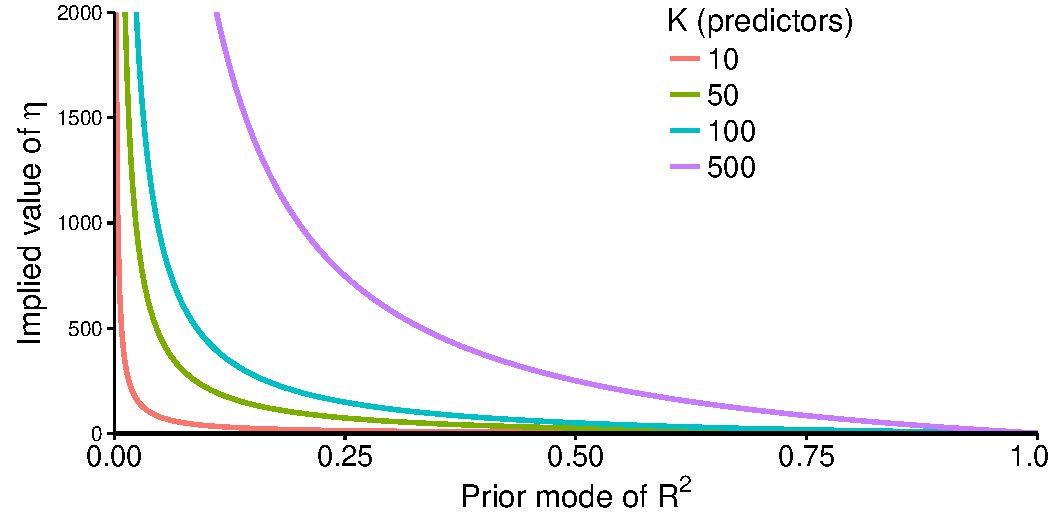
\includegraphics[width=.67\textwidth]{eta_vs_location_plot.pdf}{\vspace{-.25cm}}
\caption{\em \small The value of the shape parameter $\eta$ as a function of
the prior mode of $R^2$ for different values of $K$, the number of predictors.
In order to make the plotted curves easily visible we zoom vertically to the
region between 0 and 2000 on the $y$-axis.}
\label{fig:etavslocplot}
\end{figure}

Each of these specifications of $\locRsq$ implies a value of the shape parameter
$\eta$, which is the single hyperparameter of the joint prior on the
coefficients. Smaller values for $\locRsq$ will correspond to larger values of
$\eta$ (Figure~\ref{fig:etavslocplot}), smaller prior correlations among the
outcome and predictors, and a prior density for the regression coefficients more
concentrated around zero (Figure~\ref{fig:betaplot}).

\begin{figure}
\centering
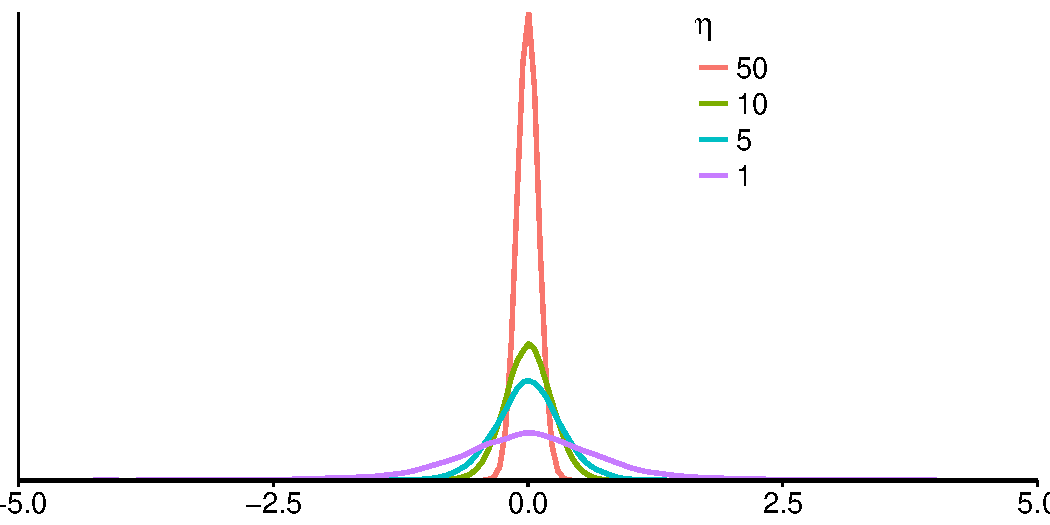
\includegraphics[width=.67\textwidth]{betaplot.pdf}{\vspace{-.25cm}}
\caption{\em \small Implied marginal prior for one of the $K$ standardized
regression coefficients (computed from 10,000 draws). Here the value of $K$ is
fixed at $100$ and the plotted densities correspond to different values of the
hyperparameter $\eta$. As the value of $\eta$ increases the prior becomes
increasingly concentrated around zero.}
\label{fig:betaplot}
\end{figure}

\subsection{Prior for the marginal standard deviation}
\label{subsec:marginalSD}
Let $\sigma_y = \omega s_y$, where $s_y$ is the sample standard deviation of the
outcome and $\omega > 0$ is an unknown scale parameter to be estimated. We use
the scale-invariant Jeffreys prior
$f_\omega \left(\omega\right) \propto 1 / \omega,$
which is proportional to a Jeffreys prior on the unknown $\sigma_y$,
$$f_{\sigma_y} \left(\sigma_y\right) \propto \frac{1}{\sigma_y}
= \frac{1}{\omega s_y} \propto \frac{1}{\omega}.$$
This is the only prior that does not contravene Bayes' theorem in this
situation, as any other prior would result in the marginal standard deviation of
the outcome being a function of the estimated standard deviation of the outcome.
This combination of parameterization and prior also makes it easy to work with
any continuous outcome variable, regardless of the unit of measurement.

When implementing the model we prefer to work with $\omega$ on the log scale
so we use the flat prior $f_\phi(\phi) \propto 1$, where $\phi =
\log{\omega}$, which is equivalent to the Jeffreys prior on $\omega$ itself. We
refer to $\phi$ as the \emph{log fit-ratio} since it is the logarithm of the
ratio of the marginal standard deviation of the outcome implied by the model to
the observed sample standard deviation,
%
$$\phi = \log{\omega} = \log{\frac{\sigma_y}{s_y}}.$$

We can interpret the log fit-ratio $\phi$ as a measure of underfitting or
overfitting. There are three general possibilities:

\begin{enumerate}
\item If $\phi = 0$, then the marginal standard deviation of
the outcome implied by the model is the same as the sample standard deviation of
the outcome  ($\sigma_y = s_y$).
\item If $\phi > 0$, then the marginal standard deviation of the outcome implied
by the model exceeds the sample standard deviation ($\sigma_y > s_y$). That is,
the model overfits the data.
\item If $\phi < 0$, then the marginal standard deviation of the outcome implied
by the model is less than the sample standard deviation  ($\sigma_y < s_y$).
Either the model underfits the data or the data generating process is nonlinear.
\end{enumerate}
%
Given the regularizing nature of the prior on \Rsq, a minor underfit would be
considered ideal if the goal is to obtain good out-of-sample predictions. If the
model badly underfits or overfits the data, then the model should be
reconsidered.

\subsection{Prior for the model intercept}
We need not directly specify a prior for $\sigmaEps$ because our prior beliefs
about $\sigmaEps$ are fully implied by our beliefs about $\omega$ and
\Rsq via the relations
%
$$ \sigmaEps = \sigma_y \sqrt{1 - R^2} = \omega s_y \sqrt{1 - R^2},$$
%
which follow from the definition of $R^2$ and the definition of $\sigma_y$ in
terms of $\omega$ and $s_y$ from Section~\ref{subsec:marginalSD}. Thus, the only
remaining distribution to specify is the prior for the model intercept
$$\alpha = \overline{y} - \overline{\mathbf{x}}^\top \R^{-1} \boldtheta.$$
As a default, a flat (improper uniform) prior $f_\alpha(\alpha) \propto 1$ is
possible as the resulting posterior distribution will be proper. Other choices
of $f_\alpha$ are also viable, for instance a zero-mean normal with scale
$\sigma_y / \sqrt{N}$.

\section{Posterior}
\label{sec:posterior}

The previous sections imply a joint posterior distribution for the primitive
parameters
$$f_{\em post}\left(\phi, \alpha, \u, R^2 \given \y, \X = \Q\R, \eta\right).$$
In Section~\ref{sec:example} we discuss sampling from this posterior using
Markov chain Monte Carlo (MCMC). Here, assume we have already obtained a sample
of size $S$ from $f_{post}$ consisting of MCMC draws
$$\left(\phi, \alpha, \u, R^2\right)^\draw
= \left(\phi^\draw, \alpha^\draw, \u^\draw, R^2^\draw\right),
\quad s = 1, \dots, S.$$
Although some of these parameters are themselves useful (e.g, the log
fit-ratio, $\phi$), we would like to make inferences with the posterior
distribution of the parameters of interest $\boldbeta$, $\sigma_y$, and
$\sigmaEps$. Following our definitions, we can obtain a sample from the
posterior of $\left(\boldbeta, \sigma_y, \sigmaEps\right)$ from the MCMC draws
of the primitive parameters by computing
%
\begin{align*}
\sigma_y^\draw &= \omega^\draw s_y = e^{\phi^\draw} s_y, \\
\sigmaEps^\draw &= \sigma_y^\draw \sqrt{1 - {R^2}^\draw}, \\
\boldbeta^\draw &= \R^{-1}\, \u^\draw \, \sigma_y^\draw
                      \sqrt{{R^2}^\draw \left(N-1\right)},
\end{align*}
%
for each draw $s = 1, \dots, S$.



\section{Example}
\label{sec:example}

\lstset{
    language=R,
    basicstyle=\footnotesize\ttfamily,
    literate={~} {$\sim$}{1}
    }

We have implemented the proposed model and prior distribution in the {\tt
stan\_lm} function in the {\tt rstanarm} R package \cite{rstanarm}. In this
section we provide a brief demonstration.

We will utilize an example from the {\tt HSAUR3} R package, which is the
companion R package to the third edition of \emph{A Handbook of Statistical
Analyses Using R} \cite{HSAUR3-book}. The model in section 5.3.1 analyzes an
experiment where clouds were seeded with different amounts of silver iodide to
see if there was increased rainfall. This effect could vary according to
covariates, which (except for time) are interacted with the treatment variable.
Most people would probably be skeptical that cloud hacking could explain very
much of the variation in rainfall and thus the prior mode of the \Rsq should be
fairly small.

The least squares estimator of this model can be replicated in R by executing

\vspace{.5cm}
\begin{lstlisting}[frame=lines]
> library(arm)  # we prefer arm's display() for printing lm() results
> data("clouds", package = "HSAUR3")
> mod <- rainfall ~ seeding * (sne+cloudcover+prewetness+echomotion) + time
> mle <- lm(formula = mod, data = clouds)
\end{lstlisting}
\vspace{.5cm}

\noindent from which we obtain the following estimated coefficients:

\vspace{.5cm}
\begin{lstlisting}[frame=lines]
> display(mle)
lm(formula = mod, data = clouds)
                                coef.est coef.se
(Intercept)                     -0.35     2.79
seedingyes                      15.68     4.45
sne                              0.42     0.84
cloudcover                       0.39     0.22
prewetness                       4.11     3.60
echomotionstationary             3.15     1.93
time                            -0.04     0.03
seedingyes:sne                  -3.20     1.27
seedingyes:cloudcover           -0.49     0.24
seedingyes:prewetness           -2.56     4.48
seedingyes:echomotionstationary -0.56     2.64
---
n = 24, k = 11
residual sd = 2.20, R-Squared = 0.72
\end{lstlisting}
\vspace{.5cm}

Note that we have \emph{not} looked at the estimated \Rsq or $\sigma$ for the
least squares model. We can estimate a Bayesian version of this model using the
{\tt rstanarm} package, which calls Stan \cite{stan} to draw from the posterior
distribution of the primitive parameters via MCMC and then uses the equations in
Section~\ref{sec:posterior} to obtain the estimates to be returned to the user.%
\footnote{The {\tt rstanarm} package is available from CRAN and source code can
be found at \url{https://github.com/stan-dev/rstanarm}. The Stan code relevant
to this paper is available in the {\tt lm.stan} file in the {\tt exec} directory.}
To fit the model we simply prepend {\tt stan\_} to the {\tt lm} call and specify
a prior mode for \Rsq using the {\tt R2} function. The {\tt what} argument to
the {\tt R2} function can take the values {\tt "mode"}, {\tt "mean"},
{\tt "median"}, and {\tt "log"}, corresponding to the four methods for
choosing $\eta$ via the specification of $\locRsq$ detailed in
Section~\ref{subsec:r2prior}.

\vspace{.5cm}
\begin{lstlisting}[frame=lines]
> library("rstanarm")
> R2prior <- R2(location = 0.2, what = "mode")
> post <- stan_lm(formula = mod, data = clouds, prior = R2prior)
> print(post)
stan_lm(formula = mod, data = clouds, prior = R2prior)

Estimates:
                                Median MAD_SD
(Intercept)                      2.5    2.2
seedingyes                       6.6    3.7
sne                              0.2    0.6
cloudcover                       0.2    0.2
prewetness                       1.6    2.8
echomotionstationary             1.3    1.5
time                             0.0    0.0
seedingyes:sne                  -1.3    1.0
seedingyes:cloudcover           -0.2    0.2
seedingyes:prewetness           -0.9    3.5
seedingyes:echomotionstationary -0.2    2.0
sigma                            2.6    0.4
log-fit_ratio                    0.0    0.1
R2                               0.3    0.1

Sample avg. posterior predictive distribution of y (X = xbar):
         Median MAD_SD
mean_PPD 4.5    2.7
\end{lstlisting}
\vspace{.5cm}

The point estimates from the Bayesian model, which are represented by the
posterior medians, appear quite different from the least squares estimates.
However, the log fit-ratio is estimated to be about $0$, which indicates a good
fit of the model to the data.%
\footnote{The uncertainty estimates labeled {\tt MAD\_SD} are proportional to
the median absolute deviation (MAD) from the posterior median. The {\tt
rstanarm} package reports {\tt MAD\_SD} rather than the raw posterior standard
deviations because the former will be more robust for long-tailed distributions.
}
It would be safe to conclude that the least squares estimator considerably
\emph{overfits} the data since there are only $24$ observations with which to
estimate $12$ parameters and no prior information is leveraged. In general, we
would expect the prior derived in this paper to be well-suited in situations
like the one above, where there are many predictors relative to the number of
observations.


\section{Conclusion}

Priors can be easy or hard for applied researchers to \emph{specify} and easy or
hard for applied researchers to \emph{conceptualize}. Traditional shortcut
priors for regression coefficients are often used because they are both easy to
specify and to conceptualize. In comparison, the informative prior on \Rsq
proposed in this paper is difficult to conceptualize, but with its
implementation in the {\tt rstanarm} package it is now equally easy to specify.

In this paper we have only focused on the most basic linear regression models.
However, the proposed framework is flexible enough to accomodate more
complicated scenarios. For instance, a natural extension would be to allow for
the stratification of observations and the shrinking of \Rsq values within each
stratum toward a common global value.%
\footnote{See, for instance, \citeA{gelman-pardoe} for an example of how \Rsq
can be defined at each level of a hierarchical model.}
We plan to implement this feature in future versions of {\tt rstanarm}.


%: References
\nocite{Rcore}
\nocite{HSAUR3-package}
\bibliography{references.bib}


%: End document
\end{document}
